\chapter{METODE PENELITIAN}

\section{Lokasi dan Waktu Penelitian}
Penelitian akan dilakukan di Palembang selama Quarter 1 tahun 2026.

\begin{ganttchart}[
    hgrid,
    vgrid,
    bar height=0.7,
    x unit=2cm,
    bar label font=\small,
    milestone label font=\small,
    group label font=\small,
    bar/.append style={fill=blue!40},
    bar incomplete/.append style={fill=gray!30},
    milestone/.append style={fill=red!60},
    group/.append style={fill=green!40}
]{1}{3}
  % Judul bulan
  \gantttitle{Januari}{1}
  \gantttitle{Februari}{1}
  \gantttitle{Maret}{1} \\

  % Aktivitas
  \ganttbar[bar/.append style={fill=blue!40}]
    {\parbox{5.5cm}{Pengumpulan dokumen, cleaning, dan Ground Truth QA}}{1}{1} \\

  \ganttbar[bar/.append style={fill=orange!40}]
    {\parbox{5.5cm}{Pengembangan Sistem RAG dan instalasi environment}}{1}{2} \\

  \ganttbar[bar/.append style={fill=green!40}]
    {\parbox{5.5cm}{Pelaksanaan eksperimen (9 skenario x 3 model)}}{2}{2} \\

  \ganttbar[bar/.append style={fill=red!40}]
    {\parbox{5.5cm}{Evaluasi metrik, analisis data, dan kesimpulan}}{2}{3}

\end{ganttchart}

% [29]

\section{Populasi dan Sampel}
% [29]
Penelitian ini menggunakan metode eksperimen kuantitatif dengan desain faktorial. Desain ini digunakan untuk menguji pengaruh variabel bebas (panjang chunk dan overlap) terhadap variabel terikat (akurasi jawaban).

\section{Jenis dan Sumber Data}
% [30]
\subsection{Sumber Data}
Penelitian ini akan menggunakan dua jenis dokumen berbeda untuk mengevaluasi kehandalan strategi \textit{chunking} dan \textit{overlap} pada berbagai jenis dokumen dengan domain yang berbeda. Dokumen yang akan digunakan sebagai \textit{Knowledge Base Document} adalah dokumen yang tersedia secara publik yaitu:

\begin{itemize}
    \item Dokumen Hukum dan Pemerintah \par
      Korpus dokumen hukum disusun dari regulasi resmi pemerintah Indonesia. Dokumen yang digunakan adalah \textbf{Undang-Undang Nomor 11 Tahun 2008 tentang Informasi dan Transaksi Elektronik (UU ITE)} dan amandemennya \textbf{Undang-Undang Nomor 1 Tahun 2024}. Dokumen ini didapatkan dari sumber resmi pemerintah melalui situs resmi Jaringan Dokumentasi dan Informasi Hukum Kementerian Komunikasi dan Digital (JDIH). Domain ini dipilih untuk menguji coba kemampuan model dalam menangani teks yang padat, formal, dan kompleks secara struktural
    \item Korpus Berita Bahasa Indonesia \par
      Selain dokumen hukum, untuk menyediakan dataset umum yang valid, peneliti juga menggunakan \textit{Indonesian News Corpus} yang merupakan kumpulan berita berbahasa Indonesia yang tersedia secara publik. Dataset ini mencakup berbagai topik dan gaya penulisan berita yang beragam, sehingga cocok untuk menguji generalisasi model pada konten non-legal. Korpus ini menjadi pelengkap yang merepresetasikan teks bahasa Indonesia yang lebih bervariasi topik dan gaya bahasa (jurnalistik), yang berbeda dengan struktur kaku dokumen hukum seperti pada dokumen UU ITE.
\end{itemize}
Dokumen dari kedua sumber tersebut kemudian digabungkan menjadi satu korpus terpadu yang akan dijadikan dasar bagi proses retrieval.

\subsection{Proses Data}
\begin{itemize}
    \item Ekstraksi: Mengambil teks dari format PDF.
    \item Pembersihan: Menghapus format HTML, header/footer yang berulang, dan karakter non-alfabetik.
    \item Pembuatan Pasangan Pertanyaan-Jawaban (QA Pairs):
    \item Sejumlah 50 pertanyaan akan dibuat berdasarkan konten dokumen.
    \item Ground Truth Hibrida:
        \begin{itemize}
            \item Manual: Peneliti membuat 20 jawaban benar secara manual untuk validasi awal.
            \item LLM-Based: Menggunakan model LLM besar (seperti GPT-4o) untuk menghasilkan 30 jawaban benar sisanya, yang kemudian diverifikasi oleh peneliti.
        \end{itemize}
\end{itemize}


\section{Metode Pengumpulan Data}
% [31] Questionnaire, Interview, Observation.
% Rencana atau strategi pengumpulan data.
\begin{itemize}
    \item \textbf{Pengumpulan Data:} Jawaban generasi dari SLM dicatat dan disimpan dalam format CSV/JSON.
    \item \textbf{Analisis Data:}
        \begin{enumerate}
            \item Menghitung skor F1, ROUGE, dan Cosine Similarity antara jawaban SML dan Ground Truth. \citep{es2025ragasautomatedevaluationretrieval}
            \item Melakukan analisis statistik deskriptif (rata-rata dan standar deviasi).
            \item Jika memungkinkan, melakukan uji ANOVA (Analysis of Variance) untuk melihat apakah perbedaan panjang chunk memberikan pengaruh yang signifikan secara statistik.
        \end{enumerate}
\end{itemize}

\section{Definisi Operasional Variabel}
% [31] Table format usually.
% Gambaran detail tentang struktur penelitian (Variabel, Dimensi, Indikator).
\begin{itemize}
  \item \textbf{Variabel Bebas:}
  \begin{enumerate}
    \item Panjang Chunk: 128 token, 256 token, 512 token.
    \item Overlap: 0\%, 10\%, 20\% dari panjang chunk.
  \end{enumerate}

  \item \textbf{Variabel Terikat:}
  \begin{enumerate}
    \item Akurasi Leksikal: F1-Score dan Recall.
    \item Akurasi Semantik: Cosine Similarity (menggunakan embedding model multilingual, misal \texttt{intfloat/multilingual-e5-large}).
  \end{enumerate}

  \item \textbf{Variabel Kontrol:}
  \begin{enumerate}
    \item Model LLM \textit{Qwen2.5-3B-Instruct, Sailor2-3B-Chat, SEA-LION-v1-3B}.
    \item Perangkat Keras (Laptop Intel Core i7 Evo, RAM 16GB, Intel Iris Xe).
    \item Temperatur generasi (diset pada 0 untuk deterministik).
  \end{enumerate}
\end{itemize}


\section{Alur Penelitian}
% [32] SPSS, Thematic, etc.
% Teknik analisis yang akan digunakan.
Peneliltian ini ditujukan untuk mengidentifikasi kombinasi optimal dari panjang chunk dan overlap yang paling efektif dalam meningkatkan akurasi respons \textit{SLM} pada sistem \textit{Retrieval-Augmented Generation (RAG)}. Pada eksperimen ini peneliti akan membandingkan performa dari tiga SLM menggunakan berbagai konfigurasi \textit{chunk} dan \textit{overlap} dalam \textit{pipeline RAG} lokal.
Secara umum, penelitian ini diawali dengan pengumpulan data dokumen publik Bahasa Indonesia, kemudian dilakukan pemrosesan teks (\textit{preprocessing}) dan pemotongan dokumen (\textit{chunking}) berdasarkan parameter yang ditentukan. Dokumen yang telah dipotong kemudian diindeksasikan ke dalam basis data vektor untuk keperluan \textit{retrieval} pada \textit{pipeline RAG}. Selanjutnya, sistem diuji dengan serangkapan pertanyaan untuk mengukur kemampuan sistem dalam mengambil informasi yang relevan dan menghasilkan jawaban yang akurat. Akhirnya, hasil dari berbagai kombinasi parameter dianalisis untuk menemukan konfigurasi yang memberikan keseimbangan terbaik antara akurasi dan efisiensi (latensi).

\begin{figure}[H]
    \centering
    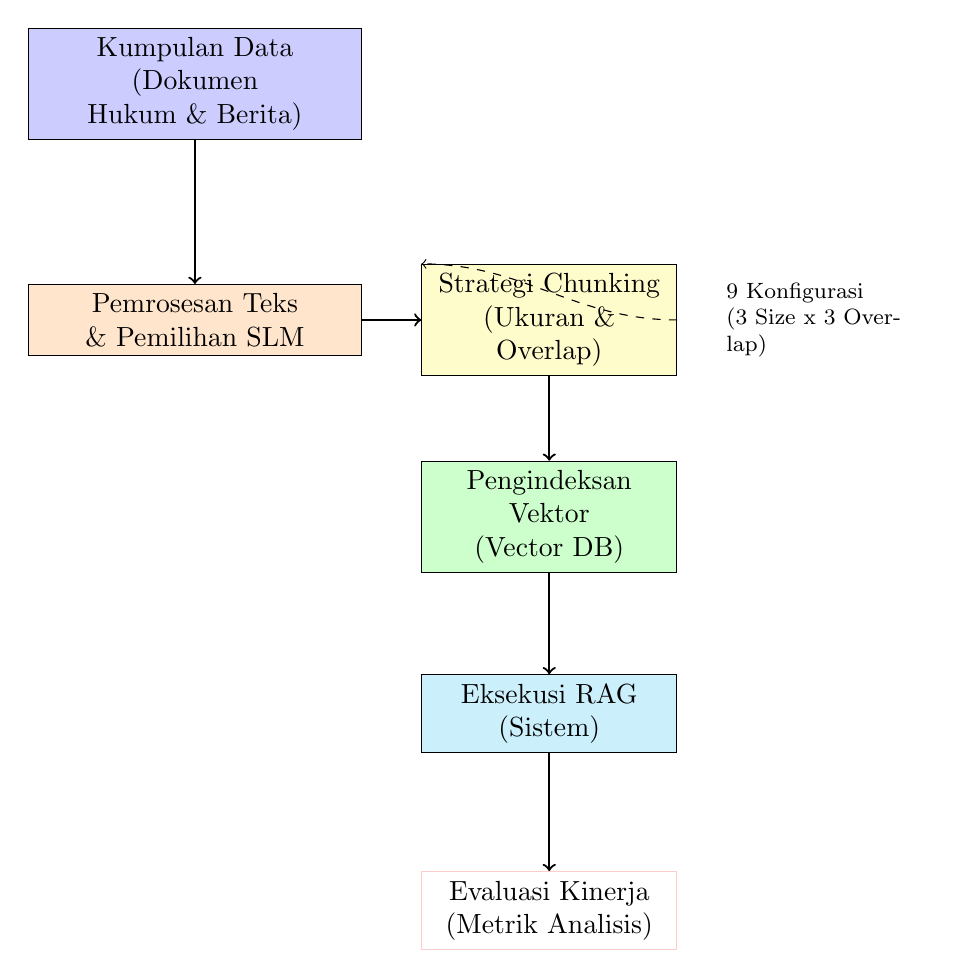
\begin{tikzpicture}[node distance=2.5cm, auto]
        % Definisi Node (Kotak-kotak)
        \node (data) [rectangle, draw, fill=blue!20, text width=4cm, align=center] {Kumpulan Data\\(Dokumen Hukum \& Berita)};
        
        \node (proc) [rectangle, draw, fill=orange!20, below of=data, yshift=-0.5cm, text width=4cm, align=center] {Pemrosesan Teks\\\& Pemilihan SLM};
        
        \node (chunk) [rectangle, draw, fill=yellow!20, right of=proc, xshift=2cm, text width=3cm, align=center] {Strategi Chunking\\(Ukuran \& Overlap)};
        
        \node (index) [rectangle, draw, fill=green!20, below of=chunk, text width=3cm, align=center] {Pengindeksan Vektor\\(Vector DB)};
        
        \node (rag) [rectangle, draw, fill=cyan!20, below of=index, text width=3cm, align=center] {Eksekusi RAG\\(Sistem)};
        
        \node (eval) [rectangle, draw, draw=red!20, below of=rag, text width=3cm, align=center] {Evaluasi Kinerja\\(Metrik Analisis)};
        
        % Definisi Panah (Hubungan)
        \draw [->, thick] (data) -- (proc);
        \draw [->, thick] (proc) -- (chunk);
        \draw [->, thick] (chunk) -- (index);
        \draw [->, thick] (index) -- (rag);
        \draw [->, thick] (rag) -- (eval);
        
        % Tambahan: Loop Parameter (Opsional untuk menunjukkan perulangan)
        \node [right of=chunk, xshift=1cm, text width=2.5cm, font=\footnotesize] {9 Konfigurasi\\(3 Size x 3 Overlap)};
        \draw [dashed, ->] (chunk.east) to [out=180,in=0] (chunk.north west);
    \end{tikzpicture}
    \caption{Diagram Alur Penelitian}
    \label{fig:alur_penelitian}
\end{figure}

\subsection{Pengumpulan Data dan Korpus Pengetahuan}
Dalam penelitian ini, digunakan dua sumber data dokumen utama untuk membentuk Korpus Pengetahuan (\textit{Knowledge Base}) bagi sistem \textit{RAG}. Pemilihan dokumen didasrkan pada representatitas teks publik di Indonesia yang sering diakses masyarakat, yaitu dokumen hukum/pemerintah dan berita.
\subsection{Pemilihan Model}
Untuk mengevaluasi performa dari SLM pada \textit{hardware} dengan sumber daya terbatas namun masih tetap mendapatkan nilai akurasi yang tinggi untuk Bahasa Indonesia, peneliti memilih 3 model dengan ukuran parameter sekitar 3 miliar (3B) yang telah dioptimalkan untuk inferensi khususnya untuk bahasa Indonesia. Model yang dipilih menyeimbangkan kemampuan multibahasa global dengan optimisasi performa bahasa khususnya bahasa-bahasa di Asia Tenggara khususnya Indonesia. Berikut 3 model yang dipilih:
\begin{itemize}
    \item \textbf{Qwen2.5-3B-Instruct:} Model ini digunakan sebagai \textit{baseline} global multilingual model. Model ini merupakan bagian dari \textit{Qwen2.5} series yang dikembangkan oleh Alibaba. Model ini telah mengalami peningkatan yang signifikan pada tahapan \textit{pre-training} dan \textit{post-training} untuk mendukung lebih dari 29 bahasa, termasuk bahasa Indonesia. Menjadikannya model SLM yang tepat sebagai referensi performa global.
    \item \textbf{Sailor2-3B-Chat:} Dipilih sebagai representasi dari model yang telah dioptimalkan khususnya untuk bahasa-bahasa di daerah Asia Tenggara. Model ini secara eksplisit mendukung bahasa Inggris, Chinese, dan bahasa-bahasa di Asia Tenggara termasuk bahasa Indonesia, bahkan bahasa Jawa dan Sunda. Hal ini sejalan dengan temuan pada penelitian sebelumnya yang menunjukkan bahwa model yang dioptimalkan untuk bahasa khusus memiliki performa yang lebih baik dibandingkan model multibahasa global \citep{cahyawijaya-etal-2021-indonlg}
    \item \textbf{SEA-LION-v1-3B:} Model ini merupakan bagian dari seri \textit{SEA-LION} yang dirancang untuk mendukung 11 bahasa di Asia Tenggara, khususnya Indonesia, Vietnam, dan Thailand. Peneliti memilih model dengan 3 miliar parameter (3B) untuk menjaga konsistensi dengan model lain yang digunakan dalam eksperimen.
\end{itemize}
Dikarenakan penelitian ini memiliki batasan pada sumber daya yang digunakan, ketiga model diatas menggunakan versi \textit{quantized (4-bit atau 8-bit)} untuk memastikan supaya dapat dioperasikan dengan batasan memori yang terbatas (RAM 16GB dan Onboard GPU), sehingga memungkinkan penggunaan model SLM secara lokal tanpa perlu akses ke \textit{cloud computing} berskala enterprise.
Eksperimen akan dilakukan dengan skema berikut:
\begin{itemize}
    \item \textbf{Sistem RAG Lokal:} Membangun pipeline menggunakan framework LangChain atau LlamaIndex.
    \item \textbf{Konfigurasi Model:} Model akan dijalankan dalam format GGUF (4-bit quantization) agar dapat dimuat sepenuhnya ke dalam RAM 16GB dan berjalan lancar di Onboard GPU (Intel Iris) menggunakan inferensi engine seperti llama.cpp atau Ollama.
\end{itemize}

\subsection{Strategi Pemotongan Teks (\textit{Chunking}) dan \textit{Overlap}}
Untuk mengatasi batasan panjang konteks (\textit{context window}) pada model SLM dan mengoptimalkan akurasi proses \textit{retrieval}, dokumen dipotong-potong menjadi beberapa bagian teks yang lebih kecil (\textit{chunk}).
\begin{itemize}
  \item Teknik Pemotongan (\textit{Chunking Strategy}): Metode pemotongan yang idgunakan adalah \textbf{\textit{Fixed-Size Chunking}} dengan pendekatan \textit{Recursive Character Splitter}. Metode ini membagi teks berdasarkan jumlah karakter dengan menghormati batasan semantik alami (seperti paragraf dan kalimat) terlebih dahulu \citep{langchain2025splitter}. Implementasi dalam penelitian ini menggunakan prioritas pemisah ganda pada baris baru (\texttt{\textbackslash n\textbackslash n}), baris baru (\texttt{\textbackslash n}), dan akhirnya spasi.
  \item Variabel Ukuran \textit{Chunk}: Penelitian ini menguji tiga konfigurasi ukuran \textit{chunk} untuk menemukan titik keseimbanganantara konteks dan presisi:
    \begin{itemize}
        \item \textbf{128 token}: Ukuran kecil yang diharapkan memberikan presisi tinggi dalam \textit{retrieval} namun memiliki risiko kehilangan konteks antar potongan.
        \item \textbf{256 token}: Ukuran menengah yang sering digunakan sebagai default dalam praktik \textit{RAG}.
        \item \textbf{512 token}: Ukuran besar yang diharapkan memberikan konteks yang lebih luas namun mungkin mengurangi presisi karena memasukkan informasi-informasi yang kurang relevan (\textit{noise}) ke dalam jawaban.
    \end{itemize}
\end{itemize}

\subsection{Variabel \textit{Overlap} (Tumpang Tindih)}
Untuk memitigasi risiko pemutusan informasi di antar batas chunk, diterapkan mekanisme overlap (perulangan teks). Tiga persentase overlap yang diuji adalah: 

\begin{itemize}
     \item 0\%: Sebagai kontrol ablasi untuk mengukur dampak pemisahan total tanpa tumpang tindih.
     \item 10\%: Persentase tumpang tindih yang direkomendasikan dalam praktik terbaik untuk menjaga koherensi konteks \citep{weaviate2024chunking}.
     \item 20\%: Tumpang tindih yang lebih besar untuk memastikan tidak ada informasi krusial yang terlewat di batas antar chunk.
\end{itemize}

Dengan kombinasi 3 ukuran chunk dan 3 persentase overlap, terdapat total 9 konfigurasi pemrosesan dokumen yang akan diuji pada setiap model. 

\subsection{Desain Sistem \textit{Retrieval-Augmented Generation (RAG)}} 

Sistem RAG yang dibangun dalam penelitian ini mengadopsi arsitektur standar yang terdiri dari tiga komponen utama: \textit{Retriever}, \textit{Knowledge Base}, dan \textit{Generator}. 

\begin{itemize}
  \item Representasi Vektor dan Pengindeksan \textit{(Vector Embedding \& Indexing)} \par
  Setiap chunk dokumen diubah menjadi representasi numerik (\textit{embeddings}) menggunakan model \textit{embedding multilingual} yang tetap untuk seluruh eksperimen. Pilihan embedding model ini bertujuan untuk memastikan bahwa perbedaan kinerja yang teramati disebabkan oleh strategi chunking atau model SLM, bukan oleh perbedaan metode retrieval. Vektor hasil \textit{embedding} kemudian disimpan dalam indeks vektor menggunakan \textit{FAISS (Facebook AI Similarity Search)} untuk memungkinkan pencarian cepat dan efisien. 
  \item Mekanisme Retrieval \par
  Saat menerima pertanyaan dari pengguna, sistem akan mengubah pertanyaan menjadi vektor menggunakan embedding model yang sama. Kemudian, sistem melakukan pencarian kemiripan (\textit{nearest neighbor search}) di dalam indeks vektor untuk mengambil top-k dokumen yang paling relevan. Dalam penelitian ini, nilai k=5 ditetapkan sebagai jumlah chunk yang akan diberikan kepada model \textit{SLM} sebagai konteks tambahan. 
  \item Generasi Jawaban (\textit{Answer Generation}) \par
  \textit{Chunk} yang berhasil diambil dan pertanyaan pengguna kemudian diformat menjadi satu prompt (\textit{prompt engineering}) yang dimasukkan ke dalam model \textit{SLM}. Model \textit{SLM} bertugas untuk membaca konteks yang diberikan dan menyusun jawaban yang relevan dan koheren berdasarkan informasi tersebut. 
\end{itemize}

\begin{figure}[H]
    \centering
    \begin{tikzpicture}[node distance=1.5cm, auto]

        \node (user) [draw, ellipse, fill=gray!30] {Pertanyaan (User Query)};
        
        \node (embed) [draw, rectangle, fill=blue!10, below of=user] {Model Embedding};
        
        \node (db) [draw, cylinder, shape border rotate=90, yshift=-1cm, aspect=0.25, fill=yellow!20, below of=embed] {Vector Database (FAISS)};
        
        \node (retr) [draw, rectangle, fill=orange!20, below of=db] {Top-K Retrieval};
        
        \node (slm) [draw, rectangle, fill=green!20, below of=retr] {Small Language Model (SLM)};
        
        \node (ans) [draw, ellipse, fill=red!20, below of=slm] {Jawaban};
        
        % Panah
        \draw [->, thick] (user) -- (embed);
        \draw [->, thick] (embed) -- (db);
        \draw [->, thick] (db) -- (retr);
        \draw [->, thick] (retr) -- (slm);
        \draw [->, thick] (slm) -- (ans);
    \end{tikzpicture}
    \caption{Arsitektur Sistem RAG}
    \label{fig:rag_vertical_fixed}
\end{figure}

\subsection{Data Pertanyaan untuk Evaluasi}

Untuk mengevaluasi kinerja sistem RAG dan dampak konfigurasi chunking penulis menggunakan 50 pertanyaan sintetis. Pertanyaan yang digunakan dibuat khusus dari korpus dokumen sendiri (UU ITE dan Korpus Berita). Pertanyaan dibuat menggunakan bantuan model bahasa besar lain yang tidak termasuk dalam evaluasi. Langkah ini penting untuk memastikan bahwa setiap pertanyaan memiliki jawaban yang eksplisit terdapat di dalam dokumen. Hal ini memungkinkan pengukuran metrik akurasi (seperti \textit{Recall} atau \textit{F1 Score}) merefleksikan kualitas strategi retrieval dan chunking, bukan sekadar ketiadaan data dalam korpus. 

\subsection{Metrik Evaluasi}

Penelitian ini menggunakan kerangka evaluasi multidimensi untuk mengukur aspek akurasi retrieval, kualitas jawaban generasi, dan efisiensi sistem. 

\begin{itemize}
  \item Metrik Tingkat Retrieval (\textit{Retrieval Metrics}) \par
    Metrik ini mengukur seberapa baik sistem dalam menemukan chunk yang relevan. 
    \begin{itemize}
        \item Recall@k: Persentase pertanyaan di mana setidaknya satu chunk yang relevan (dengan overlap token >50\% terhadap ground-truth passage) muncul dalam top-k hasil pencarian.
        \item Precision@k: Persentase chunk yang relevan di antara top-k hasil pencarian.
    \end{itemize}
     
  \item Metrik End-to-End RAG (Generasi)\par
    Untuk mengukur kualitas jawaban yang dihasilkan oleh model SLM berdasarkan konteks yang diambil, digunakan kerangka evaluasi \textit{RAGAS (Retrieval Augmented Generation Assessment)} \citep{es2025ragasautomatedevaluationretrieval}. 
    \begin{itemize}
        \item \textit{Faithfulness} (Kejujuran): Mengukur sejauh mana jawaban yang dihasilkan didukung oleh fakta yang terdapat dalam konteks yang diambil (\textit{groundedness}). Nilai \textit{faithfulness} yang tinggi menandakan rendahnya halusinasi.
        \item \textit{Answer Relevancy} (Relevansi Jawaban): Mengukur sejauh mana jawaban dihasilkan langsung menjawab pertanyaan pengguna tanpa menyimpang keluar topik.
        \item \textit{Context Precision}: Mengukur rasio sinyal-terhadap-noise pada konteks yang diambil, yaitu berapa banyak chunk yang diambil yang benar-benar relevan.
        \item \textit{Context Recall}: Mengukur kemampuan sistem untuk menemukan seluruh informasi yang diperlukan dari korpus untuk menjawab pertanyaan tersebut.
    \end{itemize}
     
  \item Metrik Efisiensi (Efficiency Metrics)\par
    Mengingat batasan perangkat keras terbatas yang digunakan (laptop standar), efisiensi sistem menjadi faktor penting. 
    \begin{itemize}
     \item Average Latency (Latensi Rata-rata): Waktu yang dibutuhkan sistem dari menerima input pertanyaan hingga menghasilkan jawaban akhir (dalam detik).
     \item Peak Memory Usage: Penggunaan memori maksimum (RAM/VRAM) selama proses inferensi untuk setiap konfigurasi.
    \end{itemize}
\end{itemize}

\subsection{Prosedur Eksperimen}
Prosedur eksperimen dilakukan secara sistematis untuk memastikan reproduktibilitas hasil. 
\begin{itemize}
    \item Persiapan dan Pemotongan Dokumen: Dokumen dari korpus hukum dan berita dipotong menggunakan skrip Python yang menerapkan \textit{Recursive Character Splitter}. Sembilan kombinasi parameter (\textit{chunk\_size}, \textit{overlap}) yaitu (128, 256, 512) token dan (0\%, 10\%, 20\%) diterapkan untuk menghasilkan set data potongan yang terpisah. 
    \item Pengindeksan Vektor (\textit{Vector Indexing}): Setiap set potongan dikonversi menjadi vektor menggunakan model embedding dan diindeksasikan menggunakan FAISS. Indeks ini disimpan untuk keperluan retrieval secara cepat. 
    \item Pelaksanaan Inferensi: Untuk setiap kombinasi parameter dan setiap model SLM, sistem dijalankan untuk memproses seluruh pertanyaan uji. Sistem mencatat log waktu (latensi) dan penggunaan memori untuk setiap eksekusi. 
    \item Koleksi Hasil dan Perhitungan Metrik: Hasil jawaban dan konteks yang diambil disimpan. Selanjutnya, metrik evaluasi (\textit{Recall}, \textit{F1}, \textit{Faithfulness}, dll.) dihitung. Untuk metrik \textit{RAGAS}, digunakan model \textit{LLM} lain yang lebih besar sebagai "judge" otomatis untuk menilai kualitas jawaban tanpa bias terhadap model \textit{SLM} yang sedang diuji. 
\end{itemize}

